\chapwithtoc{Introduction}
\label{chap:intro}

Ray tracing is a powerful image synthesis technique in 3D computer graphics, capable of simulating optical effects, such as reflection, refraction, and scattering with a high degree of visual realism. For this reason, it offers a variety of applications in the entertainment industry, it is used for product design, visual prototyping, and for creating visualizations in scientific research \cite[pp 91-128]{peddie2019ray}. Reasons for the popularity of ray tracing algorithms are the physical plausibility of its generated images as well as their simplicity and "elegance". 

The origins of ray tracing can be traced back as far as 1968. At that time, a method was invented to shade wire-framed solids by shooting random light rays from virtual light sources to the scene geometry and if an intersection would be found, placing a symbol at the intersection point \cite{appel1968some}. If enough rays would be generated, there would be a high concentration of these symbols at regions with high light intensity, which would approximate physical realism. 
A decade later, an elaboration of this idea to a shading model that takes global information into account for calculating light intensities \cite{whitted1979improved}, would revolutionize the computer graphics field.

\begin{figure}
	\centering
	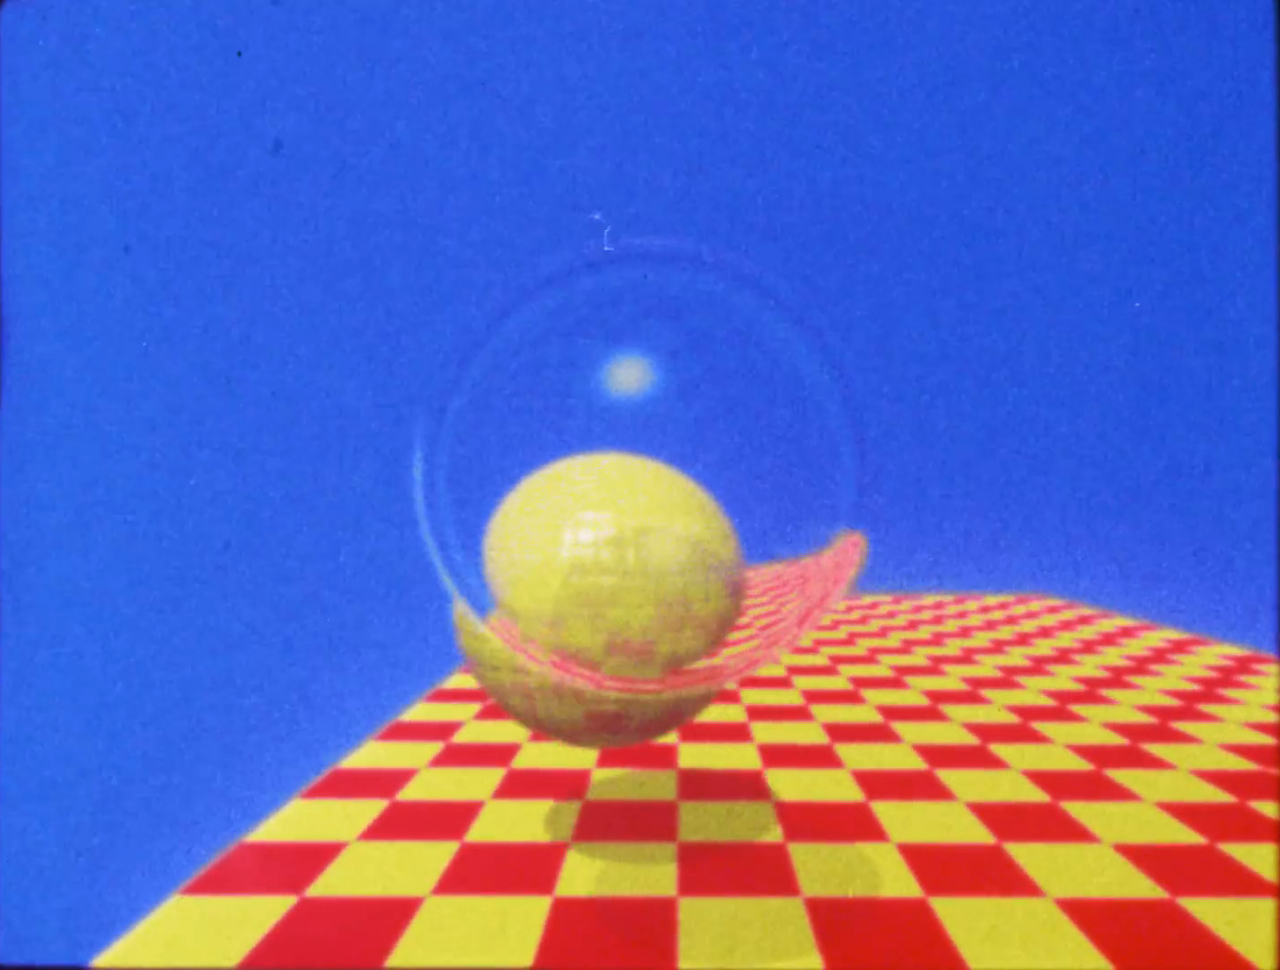
\includegraphics[width=.7\linewidth]{img/0 introduction/whitted_}
	\caption{A frame of the animation used to demonstrate the recursive ray tracer described in \cite{whitted1979improved}.\cite{raytracingvideo}}
	\label{fig:g}
\end{figure}

Over the years, novel ray tracing algorithms that were inspired by this model came to be, aiming at the increase of physical correctness in rendered images. 
However, ray tracing was and still remains a computationally demanding and therefore costly process. This is the reason much research was (and still is) devoted to the acceleration of the ray tracing procedure in order to compensate for its computational expense. A variety of ray acceleration data structures and faster intersection algorithms were introduced.
Furthermore, ray tracing is by nature is "embarrassingly parallel", meaning it is well suited for parallel processing and auto-vectorization.
As Moore's law predicted, the computational power in CPUs gradually increased. Nowadays, modern computers admit an integrated circuit with multiple cores on which the workload of the ray tracing algorithm can be distributed. While ray tracing was considered impractical during the time it was pioneered, it has now become accessible to everyone with a moderate laptop or PC, thanks to this development.

In spite of this, exploiting the computational power of modern processors to their full potential for ray tracing remains challenging. This particular reason served as the motivation for developing the award-winning (\cite{embreeAward}), open-source framework \emph{Embree} \cite{wald2014embree}. Embree offers a set of ray tracing kernels that maximize the compute capabilities of modern x86 CPU architectures. The kernels are accessible to programmers by a provided API. 

One of the design goals behind Embree was an easy integration of the framework into existing professional ray tracing engines in order to achieve high performance when ray tracing virtual scenes with high geometrical complexity.

\section*{Thesis subject and motivation}
The goal of this thesis is a successful integration of the Embree framework into the rendering engine \emph{The Advanced Rendering Toolkit} \cite{artSoftware} (which will be referred to with its abbreviation \emph{ART} throughout this thesis). ART considers its target audience computer graphics researchers. It offers innovative features, such as spectral rendering support, proper handling of bi-spectral materials (e.g. fluorescent surfaces) \cite{mojzik2018handling} and a physically plausible sky dome lighting model \cite{wilkie2013predicting}. Until the release of the Mitsuba 2 renderer \cite{nimier2019mitsuba}, ART was to our best knowledge the sole rendering system that would support rendering polarization effects. 

In order to facilitate these features, ART provides a documented scene description language which is essentially Objective-C source code (the same language ART is mostly written in) that is compiled at the beginning of a rendering process. This brings the advantage that scene geometry can be modeled by using programming concepts \todo{rephrase} such as functions and loops. The scene description language provides functionality for Constructive Solid Geometry (CSG) modeling and for importing PLY meshes as geometry objects. Furthermore, in these Objective-C scene files, one has to assemble a so-called \emph{Action Sequence}, which can be thought of as a pipeline, directing how ART processes a given scene. 
This allows for great flexibility, however, to ensure this functionality, ART relies on its very own scene description data structures, that diverge from those present in other popular rendering engines (e.g. pbrt \cite{pharr2016physically} and Mitsuba 2).

The main focus of this work is the proposing of a way to incorporate the Embree with all types of geometries one can model with ART's scene description language. Particular attention in this thesis is paid to enabling the rendering of CSG geometry with Embree. 
Although Embree was developed with the intention of it being "used in existing renderers with minimal programmer effort" \cite{wald2014embree}[p 1], this is a non-trivial task, on account of these structures and since there is no direct support for CSG geometry by Embree.

The successful integration of Embree into ART would elevate a complex image synthesis system with inimitable features regarding spectral rendering to modern ray tracing standards. \todo{Can I put it like that?}


\section*{How this thesis is structured}

This thesis is structured as follows: 

\textbf{Chapter 2} will provide fundamental background information including a brief introduction to the ray tracing technique, explanations of the most common ray acceleration structures, and an overview of both ART and the Embree framework.

In \textbf{Chapter 3}  -> my implementation

\textbf{Chapter 3} -> Evaluation and results

This work is concluded in \textbf{Chapter 4}